\paragraph{}
For this part, let's talk about a whole different beast : The software. This correspond to all of the code executed
on the microcontroller to command all of the actions done, from the control of the rocket trajectory to the log of
the temperature !

\paragraph{}
This is a very complex topic, that could be the subject of a whole report, so we're forced to reduce some part of it.
Nonetheless, we'll go trough all of the main subjects.
First, we'll talk about the configuration of the different functions by exploring the different devicetree files.
In a second time, we'll go trough the fundamentals of Zephyr RTOS, which was used to schedule main tasks and handle
the nasty memory stuff for ourselves.
Then, we'll start to ramp up into the different abstraction layers used, from the drivers to the threads.
To conlude this chapter, we're going to show the global software architecture we used over the project.

% Including all of the files
% Device trees
\section{Introduction to devicetrees}
First, we need to explain what is a devicetree, because that's actually far from begin clear and easy to understand.
The wikipedia article describe it concisely, here a quotation :

    \quote{In computing, a devicetree (also written device tree) 
    is a data structure describing the hardware components of 
    a particular computer so that the operating system's kernel 
    can use and manage those components, including the CPU or CPUs, 
    the memory, the buses and the integrated peripherals.}
    \cite{devicetree}

\paragraph{}
So, we know that we're going to found some hardware description in theses files. Theses kind of files are 
commonly used on the Linux kernel for this purpose, on hardware that is much faster than our small 
microcontroller. 
This way of describing hardware, even if it's quite difficult to get it rigth enable some extremely smart
options, such as dynamic reconfiguration.

\paragraph{}
In fact, for other controllers we're supposed to bind pins by hand by correctly assigning register values.
This is easy to develop, but once you want to change something, it become difficult to not make mistake by 
misreading a value.
This problem is solved with devicetrees, since they store hardware config for ourselves. And, they can 
even store multiple configuration, and offer the option to switch at compile time.

It's then possible to develop a devicetree for the development board, and for the final board, and within
one parameter change between them !

\paragraph{}
Devicetrees are written in plain text, and there can be only a single file used for the compilation at 
a given time. Theses files use the extension ".dts". This main file contain the root, also named "/", 
as any UNIX filesystem. Then, we add "folders", which are named nodes to it. Nodes can be 
nested inside others to make the code cleaner. Theses are sometimes called sub-nodes. And inside nodes, 
there is some properties, that can be seen as a variable that configure one aspect.

As an example, a node may be RAM, and properties are the size, the speed and any other hardware
parameters.

In correctly designed devicetrees, there shall be one node for each device that can't be detected on 
runtime. This include I2C slaves.

\paragraph{}
We can easily image that theses files will become big, even for simple systems. To give an idea, there is
arround one thousand of lines just for our simple microcontroller !

Thus, the developpers of Device Tree Compilers managed to create an include syntax, based on overlays files
(".dts\textbf{i}"). Theses are included by after and contain only the code for a single peripheral.
Then, we include them over the main devicetree file. 

If the new nodes were not present, they're added to the main code. If they were already existing, the new 
file will overhide properties. 
It's always the latest added that take the priority.




\section{Configuration using devicetrees}
Since we're using a microcontroller that is widely available, most of the work with 
devicetrees has already been done by the manufacturer.

Thus, we don't need to care about memory, cpus, or other internals details of the
peripherals. We only edit properties that are related to our needs, which include
peripherals or other ICs.

All of the structure was automatically generated by a tool provided by the manufacturer, 
that create an empty structure with everything needed to ensure the boot of the controller.

\paragraph{}
To make the structure cleaner, we've used a lot of overlays, because it's much easier
to debug and find the right property when needed.

\subsection{Main overlays}
Thus, the generated file has only a new line : the one needed to include the main overlay file.

This file look like this :

\inputminted[linenos, firstline=16, lastline=44]{devicetree}{data/code/dtc/topaze-pinctrl.dtsi}

This file is not a properly formed overlay, since it does indeed overlay nothing. But it make our
job easier by grouping all of the sub includes into a single file. Then, we can modify them for
debugging purposes.

We'll quickly move to another file that show a real overlay file, such as the PWM and I2C configuration.

\subsection{Peripherals overlays}
\subsubsection{PWM configuration}
Then, let's open a file like the PWM configuration to explore more in details what an overlay is.
For any overlay file, we used four main blocks\footnote{
    The number of block may vary depending on each architecture and software decision.
}, which are

\begin{itemize}
    \item Global peripheral configuration
    \item Pin configuration
    \item Advanced peripheral configuration
    \item Aliases
\end{itemize}

\paragraph{Global peripheral configuration} ~\\
First, we need to configure globally the peripheral.
\inputminted[linenos, firstline=17, lastline=21]{devicetree}{data/code/dtc/topaze-pwm-servo.dtsi}

Here, we're simply enabling the peripheral by setting it's status property to "okay". Then, we're 
passing a reference to a pinctrl configuration, charged to define the pins. \footnote{
    The default name is mandatory, and is used by the RTOS to know what to do with theses pins once 
    placed in low power modes. We're not using them here.
}

\paragraph{Pin configuration} ~\\
Then, right after, we're configuring the said pins. We pass a group of pins that are defined by a 
macro, that return the pin number according input like the port, the pin, and some description.

\inputminted[linenos, firstline=24, lastline=33]{devicetree}{data/code/dtc/topaze-pwm-servo.dtsi}

As previously said, we're not using low power modes so we don't need them in our project. If they 
were defined, we would see here two group of pins, one for each mode.

\paragraph{Advanced peripheral configuration} ~\\
Now, the main configuration part. That's where we configure most of the behavior of the PWM peripheral.

\paragraph{}
Before entering into the main details, we need to explain something : We created a node named "wings" here, 
that is compatible with pwm-wings. This is a custom wrote specification for our needs that wait for 
\begin{itemize}
    \item A pwm array with exactly four pwm channels
    \item A pwm period
    \item Some boundaries about the duty cycle (expressed in time domain)
\end{itemize}

\inputminted[linenos, firstline=52, lastline=66]{devicetree}{data/code/dtc/topaze-pwm-servo.dtsi}

Thus, we find here our custom node with our four servo-engines defined, and some settings.
Not all settings are used by the PWM peripheral to configure itself, but by the software that 
import them as constants.\footnote{
    For example, min-pulse and max-pulse are used by the software to compute the required 
    pulse for a defined angle.
}

\paragraph{Aliases} ~\\
Then, to conclude on this file, we define some aliases. Theses enabled the fetching of a node by quoting
it's name rather than it's location. 

\inputminted[linenos, firstline=69, lastline=74]{devicetree}{data/code/dtc/topaze-pwm-servo.dtsi}

\subsubsection{I2C configuration}
Then, in the same manner we configured the I2C \footnote{
    And a lot of other peripherals !
}. The file expose the same structure, as any overlay in the project. 

\inputminted[linenos, firstline=36, lastline=61]{devicetree}{data/code/dtc/topaze-I2C.dtsi}

The main difference with the previous file is the presence of multiple nodes here, once for each I2C sensor.
Each device can has some properties, such a compatible, status and reg properties. The last one, reg, 
correspond to it's address on the bus ! Thus, we don't care about such details on the software, we communicate
with a sensor, not a peripheral on some address.

\section{Final words}
To conclude this part, let's resume a bit the devicetree files. Theses are used for hardware related configuration, 
and expose some options that may be used to directly configure the registers of an IC, or be exposed to a C or C++ 
as constants for more advanced usage.

Theses files are complex to write, but can be used to configure precisely the differents hardware while reducing 
user errors.


% Zephyr
\section{RTOS}
For this second part, we'll go a bit higher in the software structure of the project, and see the different
layers. The first layer is the one we'll describe here, which is the RTOS.

This stand for Real Time Operating System.

    \quote{A real-time operating system (RTOS) is an operating system (OS) for real-time 
    computing applications that processes data and events that have critically defined 
    time constraints. A RTOS is distinct from a time-sharing operating system, such as 
    Unix, which manages the sharing of system resources with a scheduler, data buffers, 
    or fixed task prioritization in multitasking or multiprogramming environments. All 
    operations must verifiably complete within given time and resource constraints or 
    else fail safe. Real-time operating systems are event-driven and preemptive, meaning 
    the OS can monitor the relevant priority of competing tasks, and make changes to 
    the task priority.}
    \cite{RTOS}

\paragraph{}
Thus, we're able to specify strict time constraints for different threads. This is very usefull, since it
enable us to ensure the controller, designed for a specific sampling rate will iterate at a defined speed.

\subsection{Basic RTOS concepts}
To match they're requirements, near all of the RTOS define some basic concepts, such as :

\begin{itemize}
    \item A scheduler (that may be able to preempt a task)
    \item Some communication protocols :
    \begin{itemize}
        \item Queues
        \item Messages
        \item events
    \end{itemize}
    \item Tasks (which include a priority flag !)
\end{itemize}

\subsubsection{Scheduler}
This is the main aspect of the RTOS, because this the task responsible to schedule other tasks, 
while ensuring real times constraints. There's a lot of different architecture here, each adding
it's own set of positives or negatives aspects.

\subsubsection{Communication protocols}
For this second concepts, we need to present the differents ways to send data from one task to the 
other.

Since we're running multiple task in parallel, we can't define which instruction will be executed 
before another on another task. Thus, standard memory transfers, based on variables and pointers 
become unreliable.
In fact, most of the RTOS block theses kind of transfers !\footnote{
    The name may be different from one RTOS to the other, but the concepts remains the same. 
    Here, we used the Zephyr RTOS naming convension, as we used this RTOS by after.
}

Thus, we're forced to use thread-safe memory transfers, which are based on buffers, FIFOs and other
principle. Since the RTOS manage theses, it can enable, or disable some operations on the shared buffer.
This is done to ensure memory safety during the execution of the program.

There's indeed multiple type of transfers, depending the needs.
The first, Queues are FIFOs, and able to transfers large amount of data while ensuring the order. The 
drawback of them is they're memory footprint which can be quite large.

The second ones are similar, but only enable a small amount of data to be transfered. And, as opposed
to the FIFOs, when we overwrite the data, it's deleted rather than pushed on the Queue. It's memory
footprint is similar as the size of a single object, but, it won't enable the conservations of previous
sample. Thus, we may skip data.

The last one are Events, which are simply bit. We flip them, to notify a thread that something can, or
can't be done.

\subsubsection{Tasks}
The last concept is the Task. This correspond to a thread that is going to be executed on the CPU.
For example, a task may be the main as we know.

Since tasks are handled by the RTOS, it's possible to run multiple tasks in parallel, making control 
logic simpler. Thus, the timing logic (Timestamps...) can be removed, and replaced by a delay. The RTOS 
will then pause the task and execute another for the required duration.
\section{Zephyr RTOS}
As we seen just before, RTOS may be very usefull to create complex programs on CPUs.
Since we're using Zephyr, let's dig a bit deeper into this RTOS.

\subsection{Configuration}
As we seen previously, Zephyr isn't based on pure code to configure the device. It used 
a lot of others files, including devicetrees to describe the hardware.

This image represent the different steps to build an executable image for our chip
\begin{figure}[!hbt]
    \centering
    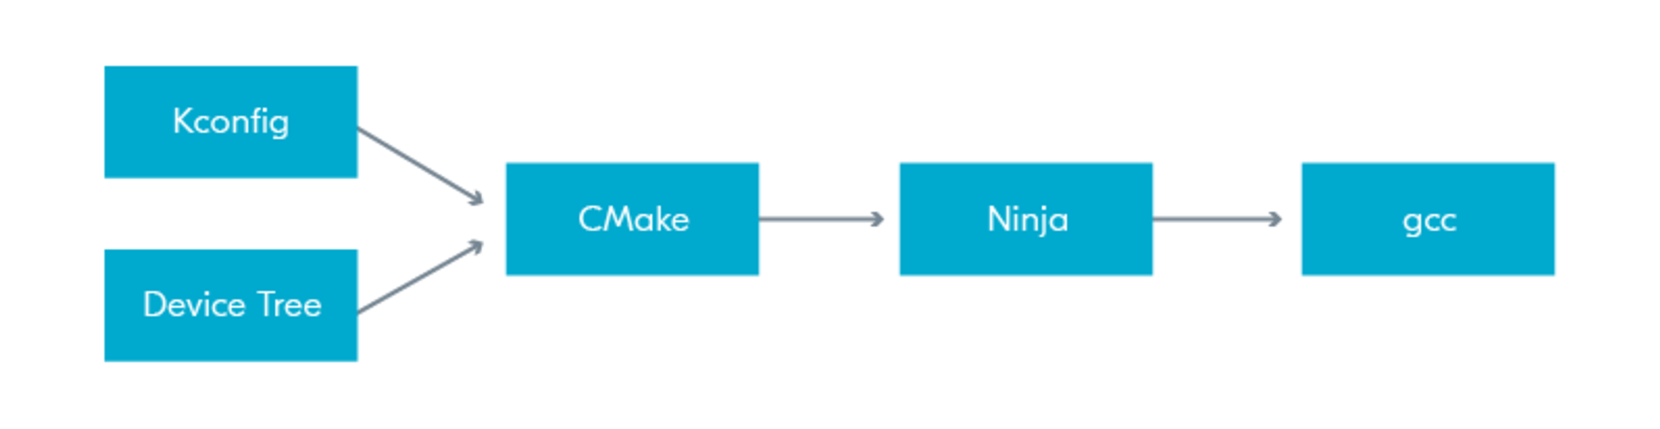
\includegraphics[width=\SchematicWidth]{images/Zephyr/ZephyrBuild.eps}
    \caption{Thread management on the Zephyr RTOS}
\end{figure}
\FloatBarrier

In this image, KConfig refer to the software configuration files, that include 
drivers selections and so. This file is linked to the devicetree, because to 
exploit a peripheral, we need to enable it in hardware, but we also need the associated
drivers with it.

To give an example, this kind of files look like : 
\inputminted[linenos, firstline=32, lastline=70]{kconfig}{data/code/cfg/prj.conf}

Thats basically a list of variable that we set to enable, or disable a software driver.

\subsection{Tasks management}
Zephyr does the task management in a different way other RTOS would. It is not bound to 
the fixed interval timer that would trigger a scheduling every period. This RTOS use the
task as self-scheduling.

\begin{figure}[!hbt]
    \centering
    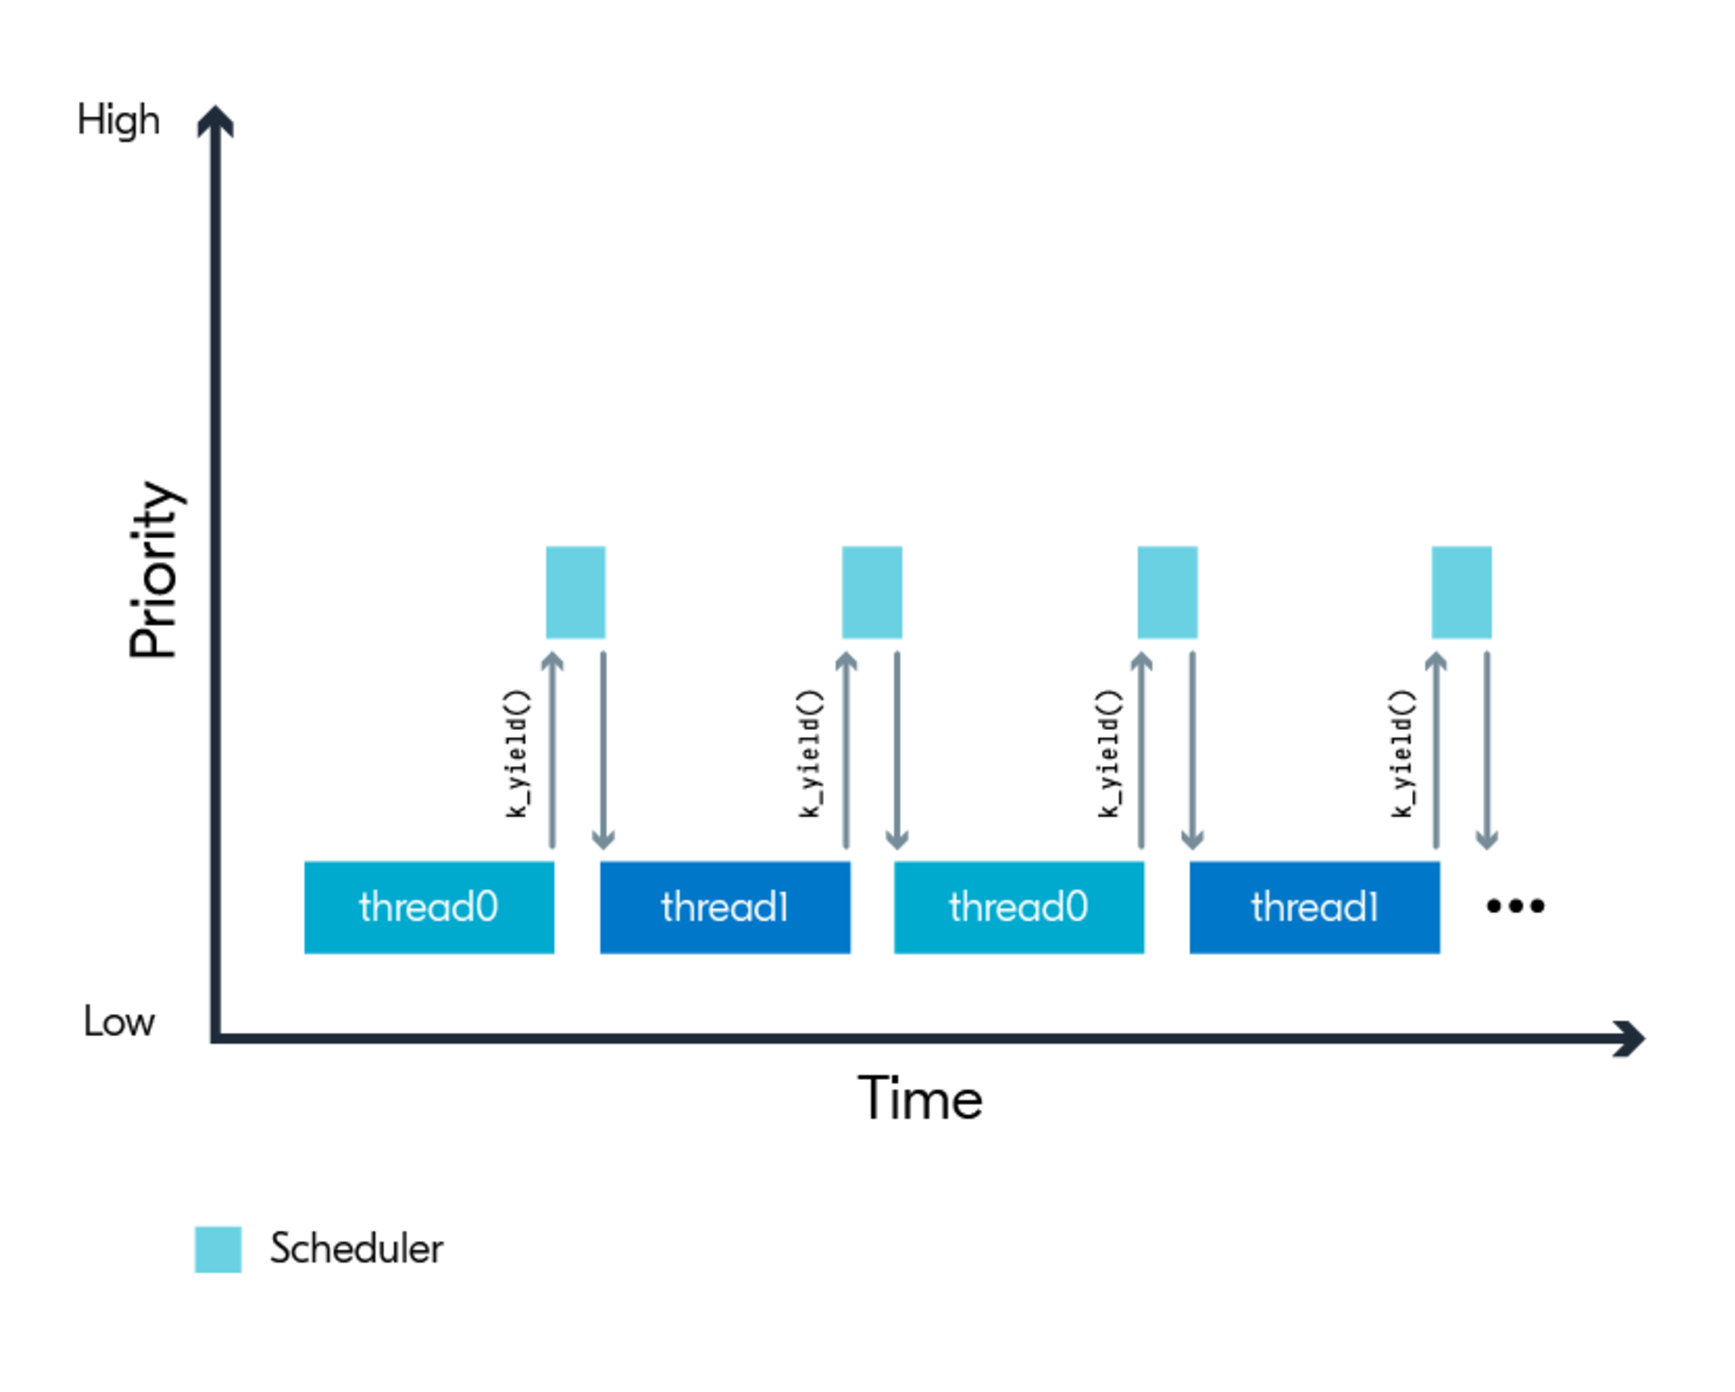
\includegraphics[width=\SchematicWidth]{images/Zephyr/ThreadMGNT.eps}
    \caption{Build chain for Zephyr RTOS}
\end{figure}
\FloatBarrier

As we may see on this image, that came from the Nordic training center \cite{NordicFundamentals} 
and \cite{NordicAdvanced} courses, the scheduler is called once a task enter a delay state, or 
yield itself.

On another hand, the RTOS include a safety timer, set to ten milliseconds that will force the
scheduler to be called. This ensure, even if a task enter an infinite loop, or crash, that
the others tasks wont crash.

\subsection{Final words}
To conclude on this RTOS part, we've seen the most basic concepts, but that's enough to
understand how our project is build, and how code interract with other code.

To sum up, Zephyr is an RTOS, used to manage a lot of different things on the project, 
from the most basic configuration of the hardware to the tasks management during the 
execution.


% Drivers
\section{Drivers}
Next in the hierarchy, we found the drivers. This codes are used to prevent from the
user to perform low-level IO, which are error prones.

\paragraph{}
All of them are written by the manufacturer or the chip, in our case, Nordic
Semiconductors.
Theses contain mostly definitions about structures passed to the driver to 
configure an element, of function that we may call.

\subsection{Calling the driver}
Theses drivers can be called by two distinct ways : 
\begin{itemize}
    \item From bare-metal code
    \item From Zephyr RTOS drivers, who redirect calls to the bare-metal code
\end{itemize}

The second method is the safest, in the manner that the RTOS handle the request for us, 
but, to ensure compatibility with a lot of chips, it can't provide exact same options as
the bare metal driver.

That's why we used both, mostly the Zephyr one were we could.

\subsection{Driver usage}
\subsubsection{Bare metal}
To give an example of the driver beeing used, there is the initialization code the ADC module 

\inputminted[linenos, firstline=103, lastline=112]{cpp}{data/code/C/saadc.cpp}

This code is responsible for the configuration of some advanced behaviors of the ADC peripheral,
such as setting it's resolution, callback function and so.
Calls are here quite long, because of the different structs that need to be configured, defined,
and applied for each aspect.

\subsubsection{Zephyr}

On the other hand, here the example for the Zephyr driver being called.
This is much simpler, because we're here calling the Zephyr Driver that handle a lot of the work 
for us, based on the devicetree !

\inputminted[linenos, firstline=100, lastline=102]{cpp}{data/code/C/servo.cpp}

We just need to care about the pulse length we want to set. All the other parameters were defined
when the kernel was booting.







\section{Device drivers}
Next, let's ramp a bit higher in the software structure. Now that we have drivers for
most simple peripherals, we'll need drivers for devices, to handle all of the specific 
protocols for us.

Thus, when we need to read a temperature, we don't want to write to a register, wait for 
some time, and then read. We want to call a function that return us the temperature.

That's the exact job for a device-driver. 
It format requests, use the peripherals drivers to handle the IO, and then make some 
calculations to return us a precise value in any cases.

These kind of drivers can be sourced from the manufacturer, but some need to be wrote by
hand. Others need to be modified to be compatible with our software decisions. Some 
other only provide standard libraries for the drivers, and let the user develop they're
own drivers.

\subsection{Manufacturer sourced drivers}
In the first case, which is the preferred option, the work needed is generally small.
For example, the driver for the IMU was entirely wrote by Bosch, which require us to 
write only the communication functions !

This look like :
\inputminted[linenos, firstline=19471, lastline=19515]{cpp}{data/code/C/bno055.cpp}

And, that's done for the driver !

\subsection{Libraries based drivers}
In this second case, the manufacturer only provided some standard libraries to be used.
An lot of work was needed to ensure this driver is correctly working. 

In the previous code section, the manufacturer provided a write and read functions to be
called. It only required us to fill them.

\inputminted[linenos, firstline=292, lastline=330]{cpp}{data/code/C/teseo.cpp}

Hopefully, manufacturer provided us some functions to check if a command was well 
formed, to match the checksum, as well as some parsers to identify the different 
elements. 

This save us a lot of time compared to writting the full driver.

In this example of code, the manufacturer provided the GNSS\_PARSER\_CheckSanity functions
and other return values codes.

We only needed to implement the IO.

\subsection{Hand written drivers}
Even if theses drivers are quite complex to write, they're generally reserved to much 
smaller chips, which make the develop quite straightforward. 
For example, the only driver we needed to develop like that was for the temperature
sensor.

\inputminted[linenos, firstline=119, lastline=158]{cpp}{data/code/C/MS5611.cpp}

This driver include all of the calculations needed for temperature corrections
needed to match the precision. Theses are indeed affected by temperature, 
or just measure range. The sensor isn't linear at all over the plage, but per 
segments.

Here, all of the code was hand written because nothing, except documentation was provided.


\subsection{Final words}
To conclude this part on drivers, we can resume them as a fundamental brick of the software, 
that handle all of the device specific requirements.
This part part is generally where the errors are, because they're difficult to test entirely.
\input{chapters/prog/HAL/API.tex}

% Gloval architecute
\section{Architecture}
For this final section on the software architecture, let's talk about the top of the pyramid.
Now, we have a fully configured chip, devices drivers, and an RTOS ready to handle task.

We just need to create the differents elements to communicate, and connect them together.

...
